\documentclass[%
 reprint,
%superscriptaddress,
%groupedaddress,
%unsortedaddress,
%runinaddress,
%frontmatterverbose, 
%preprint,
%showpacs,preprintnumbers,
%nofootinbib,
%nobibnotes,
%bibnotes,
 amsmath,amssymb,
 aps,
%pra,
%prb,
%rmp,
%prstab,
%prstper,
%floatfix,
]{revtex4-1}

\usepackage{graphicx}% Include figure files
\usepackage{dcolumn}% Align table columns on decimal point
\usepackage{bm}% bold math
\usepackage[utf8]{inputenc}
\usepackage[T1]{fontenc}
\usepackage{amsmath}
\usepackage{listings}


%\usepackage{hyperref}% add hypertext capabilities
%\usepackage[mathlines]{lineno}% Enable numbering of text and display math
%\linenumbers\relax % Commence numbering lines

%\usepackage[showframe,%Uncomment any one of the following lines to test 
%%scale=0.7, marginratio={1:1, 2:3}, ignoreall,% default settings
%%text={7in,10in},centering,
%%margin=1.5in,
%%total={6.5in,8.75in}, top=1.2in, left=0.9in, includefoot,
%%height=10in,a5paper,hmargin={3cm,0.8in},
%]{geometry}

\begin{document}

\preprint{APS/123-QED}

\title{Campos magnéticos em um cilindro supercondutor pelo modelo de London}% Force line breaks with \\

\author{Danilo Lessa Bernardineli}
\affiliation{%
 Instituto de Física, Universidade de São Paulo \\
 Rua do Matao 1371, Sao Paulo/SP, Brasil.
}%

\date{09 de ~Dezembro de 2018}
\begin{abstract}

%Ok

Neste trabalho, desenvolverá-se expressões para o potencial vetor e o campo magnético originário de um cilindro supercondutor infinito de acordo com a equação de London e de modo a rediscutir o artigo de Miguel C. N. Fiolhais e Hanno Essén ao mesmo tempo em que são feitas visualizações para a configuração do campo magnético - os quais indicam o surgimento e evolução de vórtices e turbulência internamente e externamente conforme o cilindro passa de um estado normal para um supercondutivo. Por último, são colocados ingredientes para uma eventual tentativa de caracterizar a corrente dos elétrons superfluidos no supercondutor.

\end{abstract}

\maketitle

\section{Introdução}

\subsection{Objetivos}

% Ok

Neste escrito, fará-se uma rediscussão do artigo "Magnetic field expulsion from an infinite cylindrical superconductor" dos autores Miguel C. N. Fiolhais e Hanno Essén \cite{original_article}, o qual diz respeito a dedução dos campos magnéticos externos e interiores a um cilindro supercondutor no qual as equações de London são válidas.

Os objetivos nessa rediscussão são discutir e explicitar os passos intermediários da dedução com maiores detalhes e identificar um plano de ação para caracterizar a corrente de superfluido associado ao supercondutor. Por último, é estudado a composição do campo magnético para diferentes $\lambda$.

\subsection{Modelo de London para a supercondutividade}

% Ok

O modelo de London é o primeiro modelo fenomenológico desenvolvido para um material que apresenta tanto condutividade perfeita quanto a presença do efeito Meissner-Ochsenfeld: a expulsão do campo magnético de modo que haja somente uma dependência no estado atual do sistema, sem dependência temporal em relação aos estado anterior do material. \cite{annett}.

Nesse contexto, a descrição de acordo com London foi amplamente explorada na literatura para fins didáticos devido a sua simplicidade e historicidade, sendo costumário citá-lo na introdução em livros-textos sobre supercondutividade. \cite{original_article}

O modelo de London pode ser enunciado, utilizando o formalismo do potencial vetor, como sendo expresso pela eq.  \ref{eq:vec_london}, onde $\vec{J}$ é a densidade de corrente associada a um superfluido eletrônico, $\lambda$ é o fator conhecido como profundidade de penetração de London - o qual se associa com o número de elétrons superfluidos ($n_s$) pela eq. \ref{eq:london_depth}, e $\vec{A}$ é o potencial vetor tal que o campo magnético se dá por $\vec{B} = \nabla \times \vec{A}$.  \cite{original_article} \cite{annett}

A principal hipótese de trabalho para o modelo é a tese de que na transição de um estado normal para um estado supercondutivo, uma fração dos elétrons do sólido se tornam superfluidos, o que faz com que esses elétrons se movam sem dissipação e portanto sem resistência - o que geraria um "curto circuito" e anularia a resistividade do material. Uma derivação detalhada da equação da eq. de London pode ser encontrada no livro "Superconductivity, Superfluids and Condensates", de James F. Annett. \cite{annett}

\begin{equation}
    \label{eq:vec_london}
    \vec{J}=-\frac{1}{\lambda^2}   \vec{A}
\end{equation}

\begin{equation}
    \label{eq:london_depth}
    \lambda = (\frac{m_e}{\mu_0 n_s e^2})^{1/2}
\end{equation}

% Ok

No artigo segundo Miguel e Hanno, propõe-se uma resolução detalhada do caso onde há um supercondutor cilíndrico de largura infinita e descrito pelo modelo de London de tal modo que ele tenha um raio de tamanho finito e esteja sob influência de um campo externo perpendicular ao eixo de simetria. \cite{original_article}

O resultado dos autores é a dedução do campo magnético interior e exterior ao cilindro, a dedução da componente paralela ao eixo de simetria para o potencial vetor e uma consequente discussão e visualização destes.

Nas próximas seções, irei reapresentar a solução original dos autores visando explicitar melhor os passos intermediários bem como irei apresentar uma discussão mais aprofundada acerca da configuração do campo magnético em si.

\section{Desenvolvimento}

\subsection{Formulação do sistema e condições de contorno}

% Ok

No sistema proposto, temos um cilindro supercondutor sujeito a eq. de London cujo eixo de simetria está alinhado ao eixo $\hat{z}$ com raio de tamanho R bem como um campo magnético externo $\vec{B_0}$ constante na direção $\hat{y}$ dado pela eq. \ref{eq:campo_externo}.  

\begin{equation}
    \label{eq:campo_externo}
    \vec{B_0} = B_0 \hat {y} = B_0 (\hat{\theta} \cos{\theta} + \hat{\rho} \sin{\theta})
\end{equation}

Assumindo um sistema estático e supondo a escolha de calibre para o vetor potencial como sendo a de Coulomb ($\nabla \cdot \vec{A} = 0$), teremos que a formulação potencial das equações de Maxwell serão dadas pelas equações \ref{eq:maxwell_formulation_electric} e \ref{eq:maxwell_formulation_magnetic}

\begin{equation}
    \label{eq:maxwell_formulation_magnetic}
    \nabla^2 \vec{A} + \mu_0 \vec{J} = 0
\end{equation}

\begin{equation}
    \label{eq:maxwell_formulation_electric}
     \nabla^2 V = \frac{-\rho_ e}{\epsilon_0} 
\end{equation}

Por simplicidade, ou para tornar o texto mais idêntico com o artigo rediscutido, assumirei que $\mu_0 = 1$ no restante do texto. Ademais, o vetor potencial no exterior da esfera pode ser obtido assumindo $\vec{J}=0$ (eq. \ref{eq:potencial_vetor_externo}) e no interior utiliza-se a eq. de London para a densidade de corrente, resultando na eq. \ref{eq:potencial_vetor_interno}.

\begin{equation}
    \label{eq:potencial_vetor_interno}
    \nabla^2 \vec{A} - \frac{\vec{A}}{\lambda^2} = 0, \rho \leq R
\end{equation}

\begin{equation}
    \label{eq:potencial_vetor_externo}
    \nabla^2 \vec{A} = 0, \rho > R
\end{equation}

Sendo assim, enuncia-se agora as condições de contorno, nas quais se citam quatro: A equivalência do vetor potencial para distâncias longas com o esperado diante do campo magnético externo, a continuidade do vetor potencial nas bordas do cilindro, a inexistência de correntes superficiais puras na borda do cilindro devido a existência de uma corrente interna e a regularidade do vetor potencial no interior do cilindro. As quatro condições são expressas pelas eqs. \ref{eq:contorno_distante}, \ref{eq:contorno_raio}, \ref{eq:contorno_corrente} e \ref{eq:contorno_regularidade}.


\begin{equation}
    \label{eq:contorno_distante}
     \vec{B}(\rho \rightarrow \infty) = B_0 \hat{y} = B_0 (\cos{\phi} \hat{\phi} + \sin{\phi} \hat{\rho})
\end{equation}

\begin{equation}
    \label{eq:contorno_raio}
     \vec{A}(\rho=(R + \epsilon)) = \vec{A}(\rho=(R - \epsilon))
\end{equation}

\begin{equation}
    \label{eq:contorno_corrente}
     \hat{n} \times [\vec{B}(\rho=(R + \epsilon)) - \vec{B}(\rho=(R - \epsilon))] = 0
\end{equation}

\begin{equation}
    \label{eq:contorno_regularidade}
     \vec{A}(\rho = 0) \in \mathbb{R}
\end{equation}

Por último, há a simetria do problema que faz com que o vetor potencial e o campo magnético não variem ao longo do eixo $\hat{z}$, isto é: $\frac{\partial  \vec{B}}{\partial z} = \frac{\partial \vec{A}}{\partial z} = 0$

\subsection{Resolução do sistema}

A resolução ocorrerá inicialmente desenvolvendo as expressões gerais para o potencial vetor na região interna e externa do sistema. Feito isso, serão implementadas as condições de contorno associadas ao campo externo bem como a continuidade e regularidade do sistema.

Inicia-se resolvendo o sistema para o caso livre onde o potencial vetor é dada pela eq. \ref{eq:potencial_vetor_externo}, o qual pode ser expandido em coordenadas cilíndricas na eq. \ref{eq:laplaciano_vetorial}, e que por vez possui os laplacianos expressos pela eq. \ref{eq:laplaciano_cilindrico}. Formidável.

\begin{equation}
    \label{eq:laplaciano_vetorial}
    \begin{split}
     \nabla^2 \vec{A} = &(\nabla^2 A_{\rho} - \frac{A_{\rho}}{\rho^2} - \frac{2 \partial A_{\phi} }{\rho^2 \partial \phi}) \hat{\rho} \\
    & + (\nabla^2 A_{\phi} - \frac{A_{\phi}}{\rho^2} - \frac{2 \partial A_{\rho} }{\rho^2 \partial \phi}) \hat{\phi} \\
    & + \nabla^2 A_z \hat{z} = 0
    \end{split}
\end{equation}

\begin{equation}
    \label{eq:laplaciano_cilindrico}
    \nabla^2 A_z = \frac{1}{\rho} \frac{\partial}{\partial \rho} (\rho \frac{\partial A_z}{\partial \rho}) + \frac{1}{\rho^2}\frac{\partial^2 A_z}{\partial \phi^2} + \frac{\partial^2 A_z}{\partial z^2}
\end{equation}

Felizmente, o campo magnético possui dependência somente em $A_z$, o que pode ser demonstrado ao fazer o cálculo manual pela definição e impor que não haja componente de $\vec{B}$ em $\hat{z}$. 

\begin{equation}
    \label{eq:curl_cilindrico}
    \begin{split}
    \vec{B} = \nabla \times \vec{A} = &(\frac{1}{\rho}\frac{\partial A_z}{\partial \phi} - \frac{\partial A_{\phi}}{\partial z}) \hat{\rho} \\
    &+ (\frac{\partial A_{\rho}}{\partial z} - \frac{\partial A_z}{\partial \rho}) \hat{\phi} \\
    &+ \frac{1}{\rho} (\frac{\partial (\rho A_{\phi)}}{\partial {\rho}} - \frac{\partial A_{\rho}}{\partial \phi}) \hat{z}
    \end{split}
\end{equation}

Os termos com derivadas em relação a $z$ devem ser nulos devido a condição de simetria do problema, no qual o vetor potencial não deve variar ao longo do eixo $\hat{z}$. Tem-se também a condição da componente magnética ser nula em $\hat{z}$, o que faz com que a forma de $\vec{B}$ depende somente de $A_z$, conforme a eq. \ref{eq:B_explicit}. A implementação destas condições também cria um vínculo entre $A_{\rho}$ e $A_{\phi}$, dado pela eq. \ref{eq:vinculo_curl}. Note que essa dependência utiliza somente a simetria em $\hat{z}$ como hipótese, e portanto é válido tanto no interior quanto no exterior do cilindro.

\begin{equation}
    \label{eq:B_explicit}
        \vec{B} = \nabla \times \vec{A} = \frac{1}{\rho}\frac{\partial A_z}{\partial \phi}\hat{\rho} - \frac{\partial A_z}{\partial \rho} \hat{\phi}
\end{equation}

\begin{equation}
    \label{eq:vinculo_curl}
    \frac{\partial (\rho A_{\phi)}}{\partial {\rho}} = \frac{\partial A_{\rho}}{\partial \phi}
\end{equation}

Sendo assim, pega-se um atalho para fins de calcular o campo: $\vec{A} = A_z \hat{z}$ e a eq. \ref{eq:laplaciano_vetorial} se reduz para simplesmente a eq. \ref{eq:laplaciano_cilindrico}. Porém há um custo nisso: é necessário saber todas as componentes de $\vec{A}$ para identificar $\vec{J}$ no interior do cilindro e tal tarefa está além do escopo deste escrito. Um plano de ação para tal está contido em seção posterior.

A solução para a equação de Laplace cilindrica é bem conhecida e possui a forma dada pela eq. \ref{eq:solucao_geral_exterior}

\begin{equation}
    \label{eq:solucao_geral_exterior}
    A_z = \sum_{n=0}^{\infty}[A_n cos{n \phi} + B_n \sin{n \phi}] [C_n \rho^n + D_n \rho^{-n}]
\end{equation}

O próximo passo é a aquisição de uma expressão geral para $A_z$ no interior do cilindro, que é dado pela resolução da eq \ref{eq:laplaciano_cilindrico} na eq. \ref{eq:potencial_vetor_interno}. A solução geral é apresentada pela eq. \ref{eq:solucao_geral_interior}, no qual $I_n$ e $K_n$ são as funções cilíndricas e modificadas de Bessel do primeiro e segundo tipo respectivamente. \cite{original_article}

\begin{equation}
    \label{eq:solucao_geral_interior}
    A_z = \sum_{n=0}^{\infty}[E_n \cos{n\phi} + F_n\sin{n\phi}] [G_n I_n (\rho / \lambda) + H_n K_n (\rho / \lambda)] 
\end{equation}

Estamos de posse então dos ingredientes para começar a implementar as condições de contorno. O primeiro passo é implementar a condição dada pela eq. \ref{eq:contorno_distante}, que diz respeito ao contorno quando $\rho \rightarrow \infty$. O potencial vetor que dá origem ao campo magnético externo é dado pela eq. \ref{eq:potencial_vetor_distante}, onde $A_1 C_1 = -B_0$.




% Implementar condicao de contorno distante

\begin{equation}
    \label{eq:potencial_vetor_distante}
    A_z = A_1(C_1 \rho + D_1 \rho^{-1}) \cos{\phi} + K
\end{equation}

%%%%%%%%%%%%%%%%5

O próximo passo é implementar a regularidade do potencial vetor em $\rho = 0$, o que faz com que $H_n = 0$ dado que a função modificada de Bessel do segundo tipo diverge: $K_n(\rho \rightarrow 0) \rightarrow \infty$. 

Após isso, para assegurar a continuidade de $A_z$ nas bordas do cilindro, são descartados os termos de ordem maior do que 1 na eq. \ref{eq:solucao_geral_interior} devido a independência linear dos senos e cossenos e devido a solução exterior não contê-los. Consequentemente, $A_z$ no cilindro teve ter a forma dada pela eq. \ref{eq:solucao_interior}

\begin{equation}
    \label{eq:solucao_interior}
    A_z = E_0 G_0 I_0 (\rho / \lambda) + E_1 G_1 I_1 (\rho \lambda) \cos{\phi}
\end{equation}

Novamente por independência linear dos cossenos, podemos igualar o fator do cosseno na eq. \ref{eq:solucao_interior} com o da eq. \ref{eq:potencial_vetor_distante} com $\rho = R$, o que nos dará a relação dada pela eq. \ref{eq:relacao_interior}.

\begin{equation}
    \label{eq:relacao_interior}
    \begin{split}
        &E_1 G_1 I_1 (R / \lambda) = -B_0 R + A_1 + D_1 / R \\
        &E_0 G_0 I_0 (R / \lambda) = K
    \end{split}
\end{equation}

O passo final das implementações das condições de contorno se dá pela inexistência de correntes superficiais puras (eq. \ref{eq:contorno_corrente}), o que implica na igualdade da derivada axial do potencial vetor nas bordas do cilindro, dado pela eq. \ref{eq:potencial_borda}, o qual são dados pelas eqs. \ref{eq:derivada_cilindro} e \ref{eq:derivada_exterior}.

A derivada de $A_z$ no interior é facilitada usando a relação da eq. \ref{eq:derivada_bessel}. \cite{original_article}

\begin{equation}
    \label{eq:potencial_borda}
    \frac{\partial A_z}{\partial \rho^+} = \frac{\partial A_z}{\partial \rho^-}
\end{equation}

\begin{equation}
    \label{eq:derivada_bessel}
    \frac{\partial I_v(\rho / \lambda)}{\partial \rho} = I_{v-1}(\rho / \lambda) - \frac{v \lambda}{\rho} I_v(\rho / \lambda)
\end{equation}

\begin{equation}
    \label{eq:derivada_cilindro}
    \frac{\partial A_z}{\rho^-} = E_1 G_1 [I_0(R/\lambda) - \frac{\lambda}{R}I_1(R/\lambda)] \cos{\phi}
\end{equation}

\begin{equation}
    \label{eq:derivada_exterior}
    \frac{\partial A_z}{\rho^+} = -(B_0 + \frac{A_1 D_1}{R^2})\cos{\phi} 
\end{equation}

Ao juntar tudo, é possível eliminar as variáveis $A_1, B_1, C_1, E_1 \mbox{ e } G_1$. O trabalho é longo, mas o resultado final do potencial vetor é dado pelas eqs. \ref{eq:potencial_vetor_externo_final} e \ref{eq:potencial_vetor_interno_final} para a região externa e interna respectivamente.

\begin{equation}
    \label{eq:potencial_vetor_externo_final}
    A_{z, \rho > R} = -B_0 [\rho + \frac{2 \lambda R I_0(R/\lambda) - R^2 I_1(R/\lambda)}{\rho I_1(R/\lambda)}] \cos{\phi}
\end{equation}

\begin{equation}
    \label{eq:potencial_vetor_interno_final}
    A_{z, \rho < R} = \frac{K}{I_0 (R / \lambda)} I_0(\rho / \lambda) - \frac{2 B_0 \lambda}{I_0(R/\lambda)} I_1(\rho / \lambda)
\end{equation}

Fazendo $\nabla \times \vec{A}$ no atalho dado pela eq. \ref{eq:vinculo_curl}, é possível então finalmente obtermos expressões para o campo magnéticos, dados pelas eqs. \ref{eq:campo_magnetico_interno} e \ref{eq:campo_magnetico_externo} para a região interna e externa respectivamente.

\begin{equation}
    \label{eq:campo_magnetico_interno}
    \begin{split}
        \vec{B}_{\rho>R} = &B_0 (1 - \frac{R^2}{\rho^2} + 2 \lambda \frac{R}{\rho^2} \frac{I_1(R/\lambda)}{I_0(R/\lambda)})\sin{\phi}\hat{\rho} \\
        &B_0 (1 + \frac{R^2}{\rho^2} - 2 \lambda \frac{R}{\rho^2} \frac{I_1(R/\lambda)}{I_0(R/\lambda)})\cos{\phi}\hat{\phi}
    \end{split}
\end{equation}

\begin{equation}
    \label{eq:campo_magnetico_externo}
    \begin{split}
        \vec{B}_{\rho<R} = &2B_0 \frac{\lambda}{\rho} \frac{I_1(\rho/\lambda)}{I_0(\rho/\lambda)}\sin{\phi}\rho \\
        &2B_0(\frac{I_0(\rho/\lambda)}{I_0(R/\lambda)} - \frac{\lambda}{\rho}\frac{I_1(\rho / \lambda)}{I_0(R / \lambda)}) \cos{\phi} \hat{\phi}
    \end{split}
\end{equation}



\section{Discussões}

% Ok

Com a posse da expressão do campo magnético, é possível tomar algumas direções: estudar a densidade de energia associada ao campo magnético $u_B = \frac{B^2}{2 \mu_0}$, o que foi realizado pelos autores, ou então estudar a configuração do campo magnético para diferentes $\lambda$, que é o que eu farei.

Por último, colocarei uma breve síntese de resultados que podem ser utilizados para caracterizar o potencial vetor em todas as suas componentes, o que possibilitaria identificar a corrente super fluida associada ao sistema.

\subsection{Turbulência e vórtices no campo magnético}

% Ok

Implementando as expressões do campo magnético dada pelas eqs. \ref{eq:campo_magnetico_interno} e \ref{eq:campo_magnetico_externo}, é possível fazer uma simulação com o surgimento de alguns efeitos interessantes, como vórtices de campo magnético no interior do cilindro. A simulação foi feita em um notebook online em Python3, o qual pode ser acessado e copiado em \url{https://goo.gl/rhXPRW}. Os parâmetros adotados foram de $R=1, B_0=1$ para diversos $\lambda$. A visualização foi gerada com base em recortes do domínio do campo magnético para melhorar a legibilidade da visualização. Cada sub-figura possui escala independente devido a dificuldade de visulizar os vetores em ordens de grandeza diferente.

Também coloquei as figuras em um website público (\url{https://goo.gl/ctMToJ}) para poder visualizar as imagens com maior resolução.

Os casos mais interessantes estão citados nas figuras 1, 2 e 3, os quais demonstram a variação do campo magnético conforme a variação do $\lambda$. Como $\lambda$ é associado inversamente com a quantidade de elétrons de superfluido no supercondutor, existe uma interpretação prática de que a transição de $\lambda$ maiores para $\lambda \rightarrow 0$ deve, em alguma medida, simular a transição de um estado normal para um estado supercondutivo do cilindro.

Ao visualizar as figuras, nota-se que inicialmente, para um $\lambda >> 0.5$, o campo magnético da configuração é o campo externo, porém entre $\lambda = 0.6 \mbox{ e } 0.2$, começa a surgirem vórtices e turbulências no campo tanto internamente quanto externamente, com um pico de turbulência na região externa em torno de $\lambda = 0.4$. Após isso, conforme $\lambda$ diminui para abaixo de $0.2$, a turbulência externa passa a se restringir cada vez mais próxima a borda do supercondutor, e os vórtices internos se estabilizam.

Essa turbulência é especialmente interessante pois cria-se a possibilidade de um teste experimental qualitativo para a validação do modelo de London em uma aproximação quasi-estática para a transição de fase supercondutiva. Sugere-se que o procedimento do experimento seja feito de modo que a temperatura do material oscile entre uma temperatura de estado normal e supercondutiva enquanto o campo magnético externo seja mantido constante, e se a teoria de London tiver validade,  as medições do campo magnético nas proximidades do supercondutor cilíndrico devem detectar uma turbulência transitória entre o estado inicial e final.

Por último, uma coisa notada é que o sentido do campo magnético interno inverte quase completamente de sentido em algum momento entre $\lambda=0.5 \mbox{ e } 0.4$.

Há figuras para $\lambda = 0.01, 0.2, 0.4, 0.5$ no website público (\url{https://goo.gl/ctMToJ}).

\begin{figure}[h]
    \label{fig:lambda_1}
    \caption{Campo magnético para $\lambda=1$. Nota-se que há a penetração do campo magnético por todo o cilindro.}
    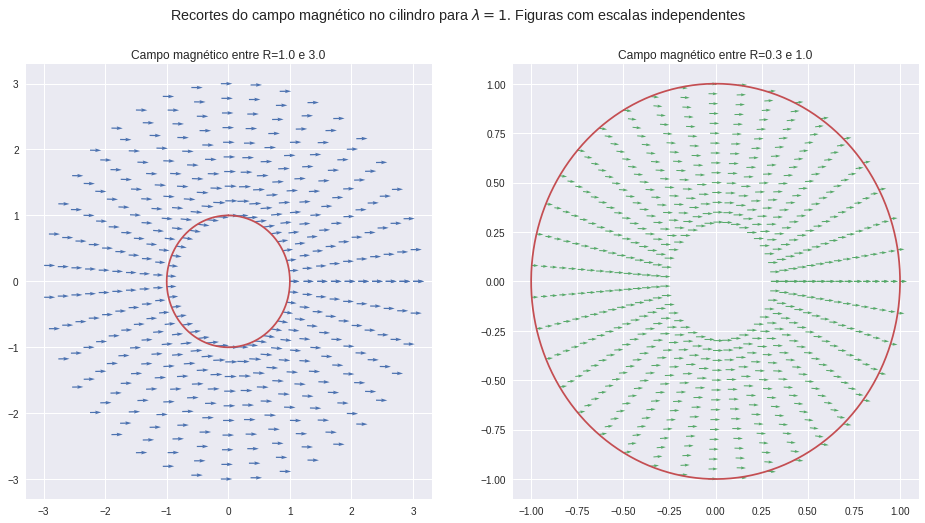
\includegraphics[width=0.49\textwidth]{lambda_1.png}
\end{figure}

\begin{figure}[h]
    \label{fig:lambda_04}
    \caption{Campo magnético para $\lambda=0.4$, que é quando começa a ter expulsão do campo magnético no supercondutor. Nota-se a turbulência gerada no entorno e o surgimento de vórtices.}
    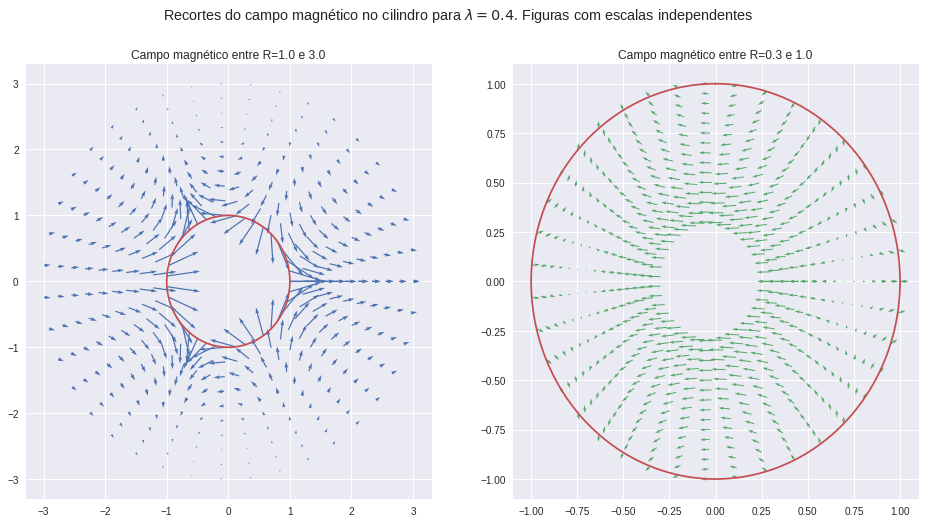
\includegraphics[width=0.49\textwidth]{lambda_04.png}
\end{figure}

\begin{figure}[h]
    \label{fig:lambda_01}
    \caption{Campo magnético para $\lambda=0.1$. Nessa situação o campo magnético interior possui vários vórtices e turbulência intensa.}
    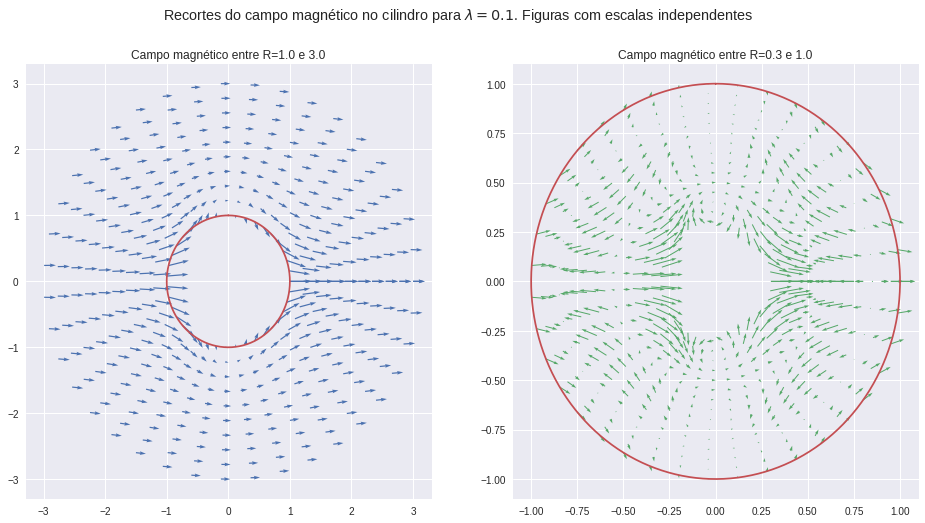
\includegraphics[width=0.49\textwidth]{lambda_01.png}
\end{figure}

\subsection{Corrente do superfluido}

% Ok

Nesta seção, colocarei alguns ingredientes que podem ser utilizados em uma eventual tentativa de deduzir o vetor potencial e por consequência a corrente de superfluido do sistema.

Para se caracterizar a corrente do superfluido dado a formulação do sistema e hipóteses de trabalho, é necessário saber todas as componentes do potencial vetor no interior do cilindro. Isso implica em resolver a eq. \ref{eq:laplaciano_vetorial} somado a um fator $-\frac{\vec{A}}{\lambda^2}$ para as componentes $A_x$ e $A_y$ usando o laplaciano da eq. \ref{eq:laplaciano_cilindrico} em coordenadas cilíndricas. Não consegui elaborar uma solução para esses casos e nem encontrar uma solução acessível na literatura.

Adicionalmente, teria-se de resolver a eq. \ref{eq:laplaciano_vetorial} para o caso livre como modo de implementar as condições de contorno dadas pelas eqs. \ref{eq:contorno_distante} e \ref{eq:contorno_raio}.

Algumas considerações podem ser usadas para obter relações visando simplificação. A primeira delas é o uso do calibre de Coulomb para obter

\begin{equation}
\label{eq:superfluido_calibre_cartesiano}
    \nabla \cdot \vec{A} = 0 \Leftrightarrow \frac{\partial A_x}{\partial x} = - \frac{\partial A_y}{\partial y} \mbox{ (coord. cartesiana)}
\end{equation}

\begin{equation}
    \label{eq:superfluido_calibre_cilindrico}
    \nabla \cdot \vec{A} = 0 \Leftrightarrow \frac{\rho \partial A_{\rho}}{\partial \rho} = - \frac{\partial A_\phi}{\partial \phi} \mbox{ (coord. cilíndrica)}
\end{equation}

O fato também de que somente $A_z$ é relevante para obter o campo magnético, impõe um segundo vínculo.

\begin{equation}
    \label{eq:superfluido_campo}
    \frac{\partial A_y}{\partial {x}} = \frac{\partial A_{x}}{\partial y}
     \mbox{ (coord. cartesiana)}
\end{equation}

\begin{equation}
    \label{eq:superfluido_campo}
    \frac{\partial (\rho A_{\phi)}}{\partial {\rho}} = \frac{\partial A_{\rho}}{\partial \phi} 
     \mbox{ (coord. cilíndrica)}
\end{equation}

Em cartesiano, é possível expressar o gradiente de $A_x$ e $A_y$ como sendo conjugados:

\begin{equation}
    \begin{split}
    &\nabla A_x = (-\frac{\partial A_y}{\partial y}, \frac{\partial A_y}{\partial x}, 0) \\
    &\nabla A_y = (\frac{\partial A_x}{\partial y}, -\frac{\partial A_x}{\partial x}, 0)
    \end{split}
\end{equation}

\section{Conclusões}

% Ok

A exploração direta da configuração vetorial do campo magnético resultante permitiu visualizar o surgimento de vórtices e de uma turbulência para diferentes $\lambda$, o que é um fenômeno curioso por si só. Dada a associação inversa de $\lambda$ com o número de elétrons superfluidos segundo o modelo de London, tal turbulência pode ser utilizada como teste experimental quanto ao domínio de validade da teoria para uma transição de fase supercondutora quasi-estática.

Uma continuidade natural desse trabalho seria de buscar caracterizar a corrente de superfluido, o que não é trivial matematicamente e ao mesmo tempo não foi possível encontrar referências sobre a realização de tal na literatura atual.

\begin{thebibliography}{9}

\section{Referencias}

\bibitem{original_article}
Magnetic field expulsion from an infinite cylindrical superconductor, Miguel C.N. Fiolhais, Hanno Essén

\bibitem{annett}
Superconductivity, Superfluids and Condensates. James F. Annett. Cap 1, pgs 2-22.

\end{thebibliography}


\section{Apêndice}

\subsection{Código para geração de imagens}

\begin{tiny}
\begin{lstlisting}[language=Python]

# Dependencias
from scipy.special import jv as I
import numpy as np
import matplotlib.pyplot as plt

# Parametros de simulacao
R = 1
B_0 = 1

def B_exterior(rho, phi, lamb=0.1):
  t_1 = 1
  t_2 = (R ** 2) / (rho ** 2)
  t_3 = 2 * lamb * R / (rho ** 2)
  t_3 *= I(1, R / lamb) / I(0, R / lamb)
  B_rho = B_0 * (t_1 - t_2 + t_3) * np.sin(phi)  
  B_phi = B_0 * (t_1 + t_2 - t_3) * np.cos(phi)
  return (B_rho, B_phi)
  
def B_interior(rho, phi, lamb=0.1):
  termo = (lamb / rho) * I(1, rho / lamb) / I(0, R / lamb)
  B_rho = 2 * B_0 * termo * np.sin(phi)
  B_phi = I(0, rho / lamb) / I(0, R / lamb)
  B_phi += -termo
  B_phi *= 2 * B_0 * np.cos(phi)
  return (B_rho, B_phi)
  
# So uma funcao auxiliar
def generate(R_min, R_max, func, N_rho=10, N_phi=40, lamb=0.1):
  rhos = np.linspace(R_min, R_max, N_rho)
  phis = np.linspace(0, 2 * np.pi, N_phi)

  phi, rho = np.meshgrid(phis, rhos)
  B = func(rho, phi, lamb=lamb)
  B_rho = B[0]
  B_phi = B[1]
  
  x = rho * np.cos(phi)
  y = rho * np.sin(phi)
  B_x = B_phi * np.cos(phi) + B_rho * np.sin(phi)
  B_y = -B_phi * np.sin(phi) + B_rho * np.cos(phi)
  
  return (x, y, B_x, B_y)
 
# Gerar a borda do cilindro 
theta_circulo = np.linspace(0, 2 * np.pi, 500)
x_circulo = R * np.sin(theta_circulo)
y_circulo = R * np.cos(theta_circulo)

# Mude a vontade
lamb = 0.1

f, axes = plt.subplots(1,2, figsize=(16, 8))
for ax in axes:
  ax.plot(x_circulo, y_circulo, color="C2", label="Borda do cilindro")
  
B_externo = generate(R, 3 * R, B_exterior, lamb=lamb)
(x, y, B_x, B_y) = B_externo
axes[0].set_title("Campo magnetico entre R=1.0 e 3.0")
axes[0].quiver(x, y, B_x, B_y, color="C0")

B_interno = generate(0.3 * R, R, B_interior, lamb=lamb, N_rho=15)
(x, y, B_x, B_y) = B_interno
axes[1].set_title("Campo magnetico entre R=0.3 e 1.0")
axes[1].quiver(x, y, B_x, B_y, color="C1")

#B_interno = generate(0.2 * R, 0.7 * R, B_interior, lamb=lamb)
#(x, y, B_x, B_y) = B_interno
#axes[2].set_title("Campo magnetico entre R=0.7 e 0.2")
#axes[2].quiver(x, y, B_x, B_y, color="C1")

plt.suptitle("Recortes do campo magnetico no cilindro para $\\lambda={}$. Figuras com escalas independentes".format(lamb))
plt.show()
\end{lstlisting}
\end{tiny}

\subsection{Imagens adicionais para o campo magnético}

\begin{figure}[h]
    \caption{Campo magnético para $\lambda=1$}
    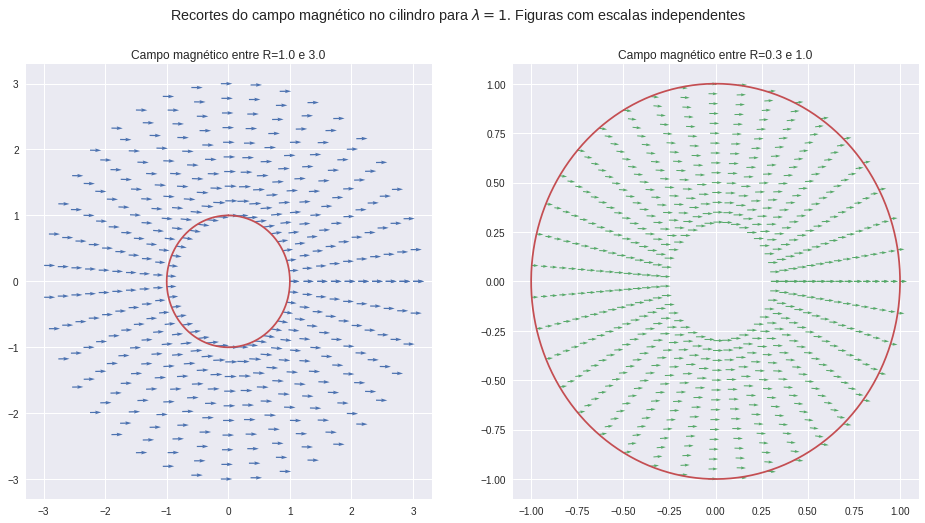
\includegraphics[width=0.99\textwidth]{lambda_1.png}
\end{figure}

\begin{figure}[h]
    \caption{Campo magnético para $\lambda=0.5$}
    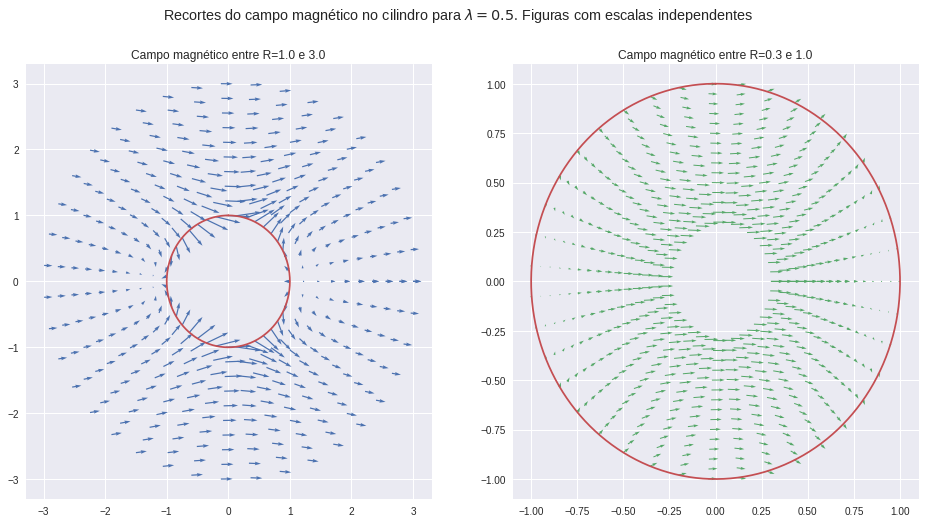
\includegraphics[width=0.99\textwidth]{lambda_05.png}
\end{figure}

\begin{figure}[h]
    \caption{Campo magnético para $\lambda=0.4$}
    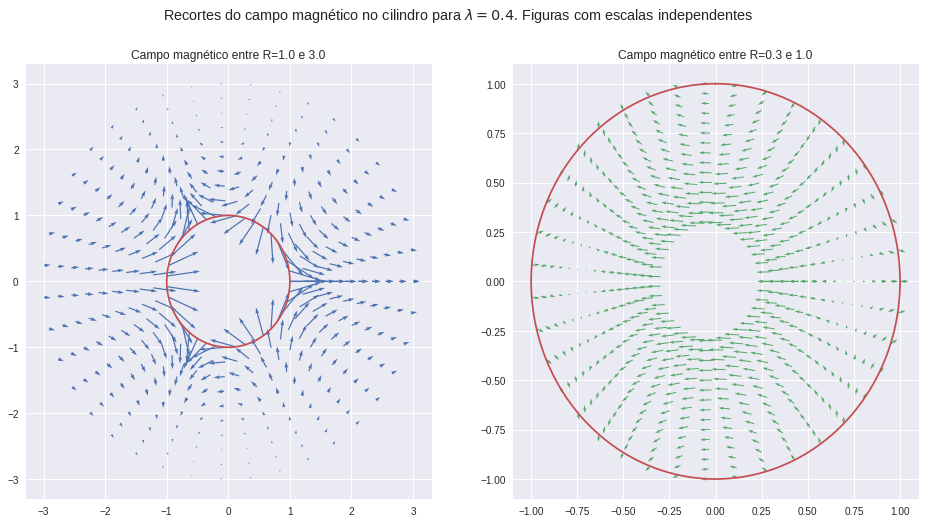
\includegraphics[width=0.99\textwidth]{lambda_04.png}
\end{figure}

\begin{figure}[h]
    \caption{Campo magnético para $\lambda=0.3$}
    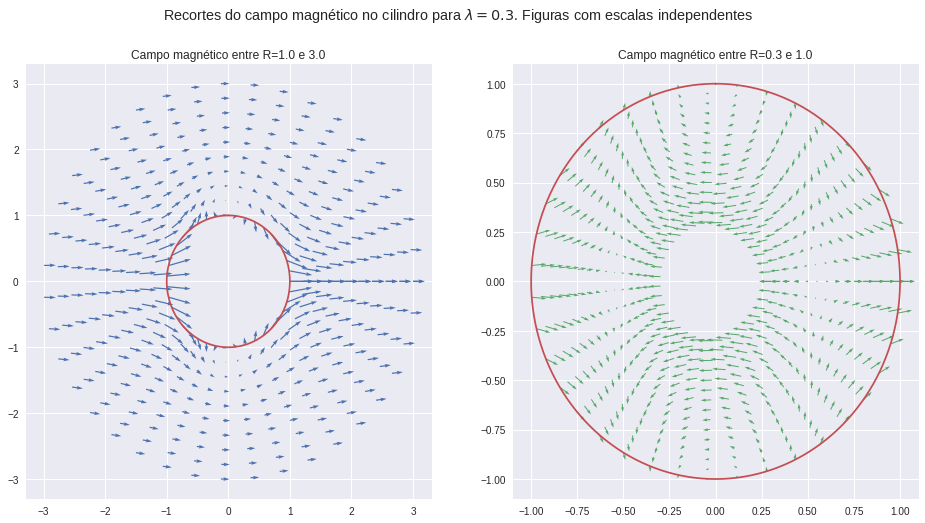
\includegraphics[width=0.99\textwidth]{lambda_03.png}
\end{figure}

\begin{figure}[h]
    \caption{Campo magnético para $\lambda=0.2$}
    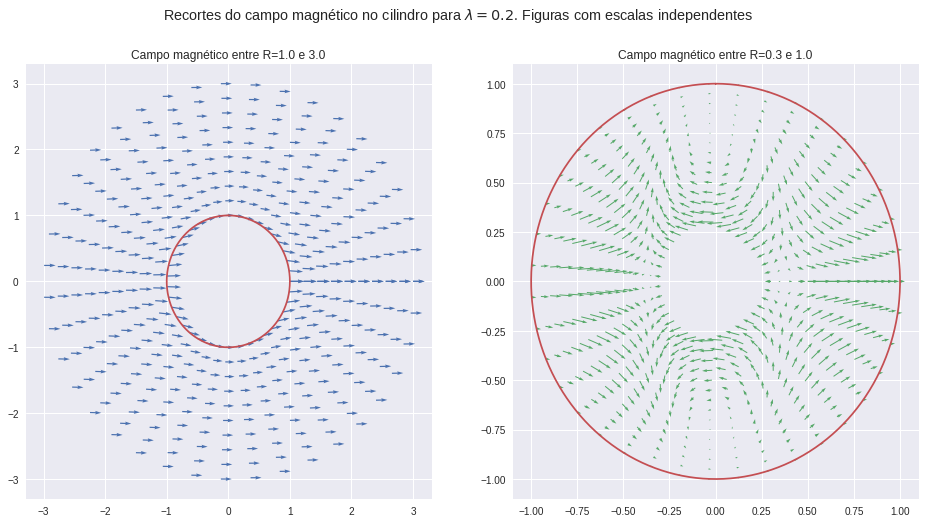
\includegraphics[width=0.99\textwidth]{lambda_02.png}
\end{figure}

\begin{figure}[h]
    \caption{Campo magnético para $\lambda=0.1$}
    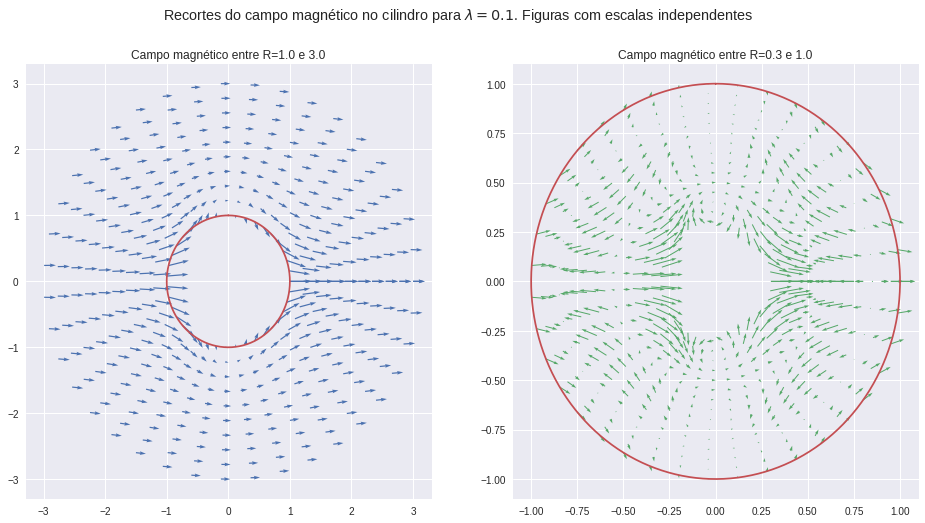
\includegraphics[width=0.99\textwidth]{lambda_01.png}
\end{figure}

\begin{figure}[h]
    \caption{Campo magnético para $\lambda=0.01$}
    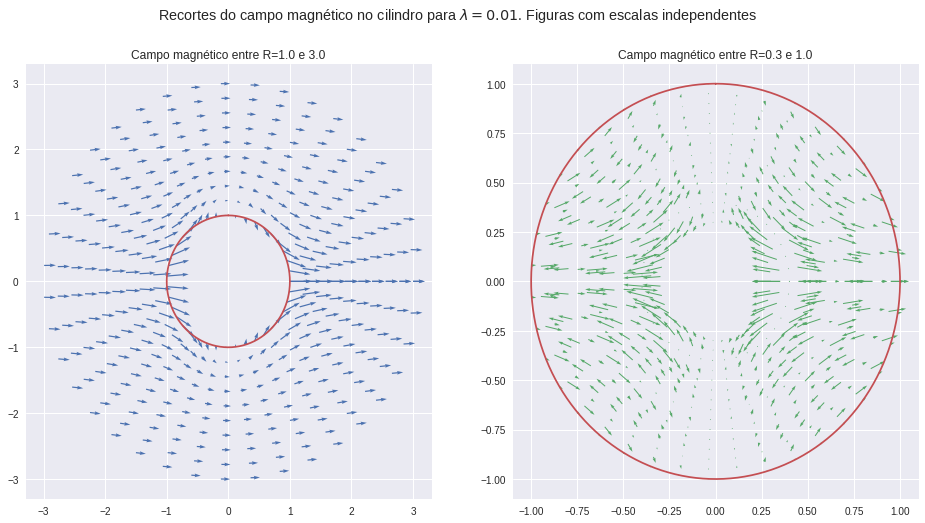
\includegraphics[width=0.99\textwidth]{lambda_001.png}
\end{figure}

\end{document}

